
\documentclass[12pt]{article}
\usepackage[paper=letterpaper,margin=2cm]{geometry}

\usepackage{amsmath}
\usepackage{amsthm} %needed for the proofs 
\usepackage{amssymb}
\usepackage{titling}
\usepackage{thmtools}
\usepackage{mathptmx} %font
\usepackage{verbatim} % for comments
\usepackage{mdframed}
\usepackage[linesnumbered,ruled,vlined]{algorithm2e}
\usepackage{lipsum}

\usepackage[T1]{fontenc} %header
\usepackage[utf8]{inputenc}%header
\usepackage{geometry} %header
\usepackage{fancyhdr}%header

%images
\usepackage{graphicx}
\graphicspath{ {./images/} }
% to include an image, do: 
%    \begin{center}
%    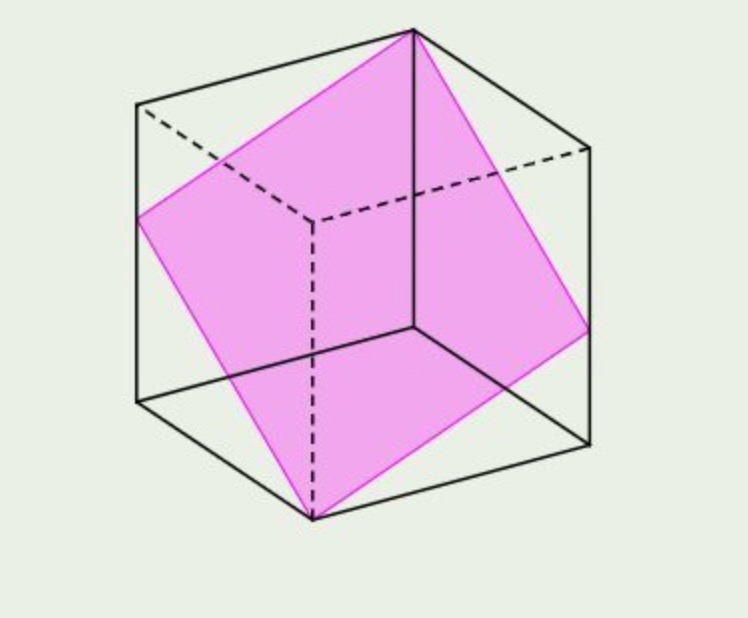
\includegraphics[scale=0.20]{graph.jpg}
%    \end{center}
% OR: 
%\begin{figure}
%    \centering
%    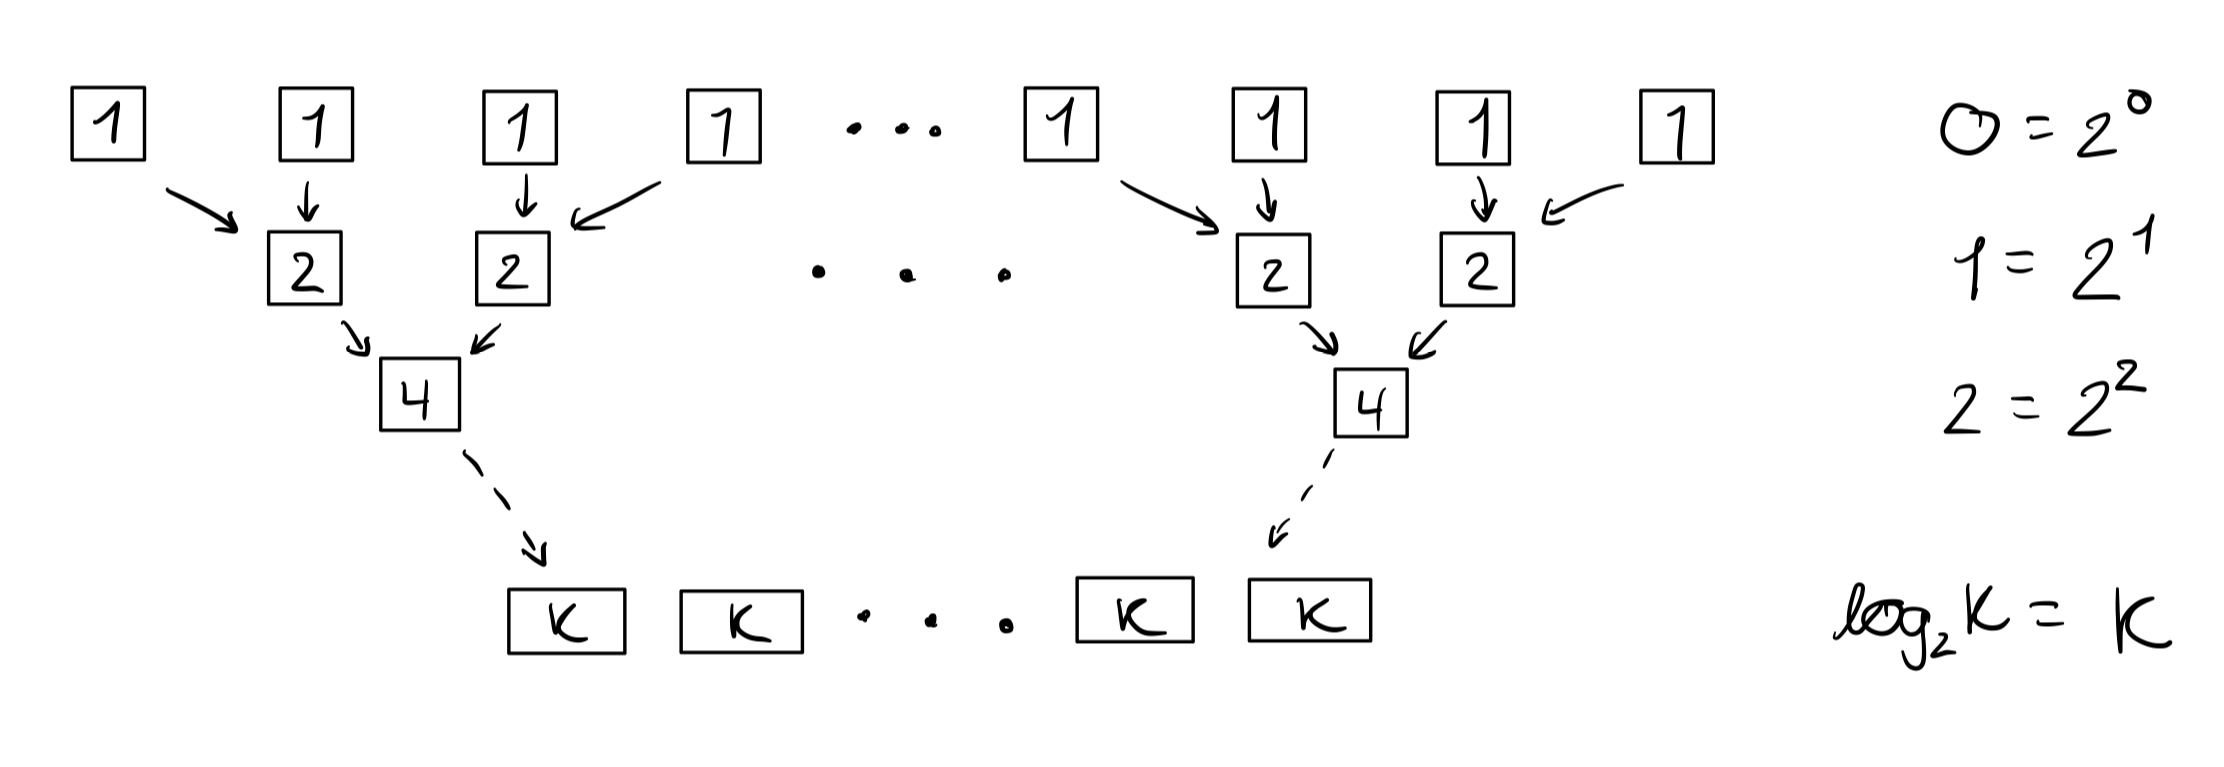
\includegraphics[scale=0.20]{IMG_1052.jpg}
%    \caption{Your caption text here.}
%\end{figure}


%macros for recursive functions
%For plots
\usepackage{pgfplots}
\pgfplotsset{compat = newest}

\newtheorem{theorem}{Theorem}
\declaretheoremstyle{lemma}
\declaretheorem[style=lemma, name=Lemma]{lemma}

\theoremstyle{definition}
\newtheorem{definition}{Definition}

\declaretheoremstyle{example}
\declaretheorem[style=example, name=Example]{example}

\theoremstyle{remark}
\newtheorem*{remark}{Remark}

\declaretheoremstyle{proposition}
\declaretheorem[style=proposition, name=Proposition]{proposition}

\declaretheorem[name=Note]{note}
\declaretheoremstyle{note}

\setlength\parindent{24pt}%set paragraph indent

\newenvironment{ftheo}
  {\begin{mdframed}\begin{theorem}}
  {\end{theorem}\end{mdframed}}


  % --- Special commands --- %
\newcommand\sol{%
  \\ 
  \\
  \textit{Solution:}\\%
}
% Statistics
\newcommand{\indep}{\perp \!\!\! \perp}
\DeclareMathOperator{\var}{Var}
\DeclareMathOperator{\cov}{Cov}

%Convex optimisation operators
\DeclareMathOperator{\cl}{cl}
\DeclareMathOperator{\epi}{epi}
\DeclareMathOperator{\lev}{lev}
\DeclareMathOperator{\dom}{dom}
\DeclareMathOperator{\aff}{aff}
\DeclareMathOperator{\ri}{ri}
\DeclareMathOperator{\argmin}{argmin}

% --- Header --- %
\renewcommand{\headrulewidth}{.4mm} % header line width

\pagestyle{fancy}
\fancyhf{}
\fancyhfoffset[L]{1cm} % left extra length
\fancyhfoffset[R]{1cm} % right extra length
\rhead{\today}
\lhead{\it Alexandre St-Aubin \& Dylan Telio}
\rfoot{}

% --- Title Page --- % 
\setlength{\droptitle}{-6em}

\title{\textsc{Assignment 3 -- COMP 252}}  
\author{\it Alexandre St-Aubin and Dylan Telio}
\date{\today}

\begin{document}
\maketitle 
\begin{enumerate}
  \item \textsc{Decision tree lower bound.}
  \begin{enumerate}
    \item[\it (i)]Give a simple algorithm for this problem and an upper bound on the complexity. For n = 5, your answer should be 7.
    \sol
    \begin{algorithm}
    \caption{An algorithm to classify the $n$ monkeys. }
    \SetKwRepeat{Do}{do}{while} %do-while loop macro
    \SetKwInput{KwOut}{Output}
    \SetKwInput{KwIn}{Input}
    \SetKwData{monk}{Monkeys}
      \SetKwData{app}{append}
    \SetKwData{typea}{Species\_1}
    \SetKwData{typeb}{Species\_2}
    \SetKwData{typec}{Species\_3}
    \KwIn{An array \monk of monkeys.}
    \KwOut{Three arrays separating the monkey species.}
    \BlankLine
    \typea $\leftarrow$ new Array;  \\ 
    \typeb $\leftarrow$ new Array;  \\ 
    \typec $\leftarrow$ new Array;  \\ 
    $i \leftarrow 1;$\\ 
    $\typea.\app(\monk[0])$;\\
      \While{$\monk[0] = \monk[i]$}{
        $\typea.\app(\monk[i])$; \\ 
        $i++;$\\ 
      }
      \tcp{loop above exits only if a second monkey species was found}
      $\typeb.\app (\monk[i]);$
    \BlankLine 
      \tcp{for each remaining monkey, compare to the 2 known species}
      \For{$j$ in range $[i, n]$ }{
      \If{$\monk[j] = \typea[0]$}{
      \typea.\app(\monk[j]);
      }\ElseIf{$\monk[j] = \typeb[0]$}{
      \typeb.\app(\monk[j]);
      }\Else{
      \typec.\app(\monk[j]);
      }
      }
  \end{algorithm}
    \begin{remark} 
      The worst case for the above algorithm is when the two first monkeys are different, and each remaining monkey is of the third or second species, hence must be compared twice (once to each of the first two species), in order to be classified. This yields a complexity of $1 + 2(n-2).$ When $n = 5, $ this is indeed equal to 7.

    \end{remark} 
    \item[\it (ii)] Show that all leaves in the decision tree must be different (i.e., correspond to different outputs).
    \item[\it (iii)] Using a decision tree-based method, show that the lower bound for this problem is 6 when $n = 5$.
    \item[\it (iv)] For general $n,$ show that the decision tree lower bound is at least $an- b$ and at most $an + b$
    for $n \geq n_0$, for some positive numbers $a, b, n_0$. Determine suitable values for these numbers. Compare this with your answer in \textit{(i)} and conclude that the decision tree bound for this problem is rather weak.
  \end{enumerate}
  \newpage
  \item \textsc{Adversarial lower bound.}
  \newpage
  \item \textsc{Lower bounds by the method of adversaries, and an algorithm.}

\end{enumerate}
\end{document}
